
% introduction to cgal

The CGAL library is a joint effort between nine European
institutes~\cite{fgkss-dccga-00}. The goal of CGAL is to make
available to users in industry and academia some efficient solutions
to basic geometric problems developed in the area of computational
geometry in a C++ software library.\\

% motivations

CGAL features a 3D polygon surface mesh data structure based on the
concept of halfedge data structure~\cite{k-ugpdd-99}, which has been
very successful for the design of general algorithms on meshes. In
this document we provide a tutorial to get started with CGAL
Polyhedron data structure through the example of subdivision
surfaces. We also offer an application both under windows and linux,
featuring an OpenGL-based viewer, an arcball for interaction and two
ways (raster and vectorial) to produce pictures and illustrations.\\

% teaser

\begin{figure}[htb]
    \centering{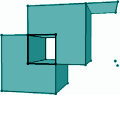
\includegraphics[width=12.0cm]{figs/teaser}}
    \caption{Snapshot taken from the tutorial application running
             on Windows. A polygon mesh is subdivided using the
             quad-triangle subdivision scheme~\cite{sl-qts-02}.}
    \label{fig:teaser}
\end{figure}
        

% targeted audience ?

The main targeted audience is a master or a Ph.D. student in computer
graphics or computational geometry, aiming at doing some research on
mesh processing algorithms. We hope this tutorial will convince the
reader~:

\begin{itemize}

\item 
not reinventing the wheel. Taking some time choosing the ``right
tool'' is often worth it. This may true, even for a short project;

\item 
using an optimized and robust library to ease the implementation and
obtain fast and robust results. This allows focusing on the elaborated
algorithm, not on the underlying data structure;

\item 
using generic programming to reuse existing data structures
and algorithms;

\item 
using a standard library in order to benefit from existing support and
discussion groups\footnote{see the cgal discuss list:
\href{http://www.cgal.org/user_support.html}
{http://www.cgal.org/user\_support.html.}}.

\end{itemize}               
